%\documentclass[xcolor=dvipsnames]{beamer}
\documentclass{standalone}

%\setbeamertemplate{navigation symbols}{}%remove navigation symbols
\usepackage{stmaryrd}
\usepackage{amssymb,amsthm,amsmath,amsxtra}
\usepackage{tikz}
\usetikzlibrary{arrows,calc,automata,shadows,backgrounds,positioning,intersections,fadings,decorations.pathreplacing,shapes,decorations,matrix}

\newcommand{\PP}{\mathbb P}

\begin{document}

    \begin{tikzpicture}%[scale=.36]
      % upstairs
      \node at (0,5) (dessin-top)
      {
        \begin{tikzpicture}[
            %scale=1,
            node distance=1.75cm,
            vblack/.style={circle,draw=black,fill=black,thick},
            vwhite/.style={circle,draw=black,fill=white,thick}
          ]
          %\node[vwhite] (A) {};
          %\node[right=of A, vblack] (B) {};
          %\node[right=of B, vwhite] (C) {};
          %\node[right=of C, vblack] (D) {};
          %\draw[thick] (A) to node [above] {} node {} (B);
          %\draw[thick] (B) to node [above] {} node {} (C);
          %\draw[thick] (C) to node [above] {} node {} (D);
          \node[vblack] (A) {};
          \node[right=of A, vblack] (B) {};
          \node[right=of B, vwhite] (C) {};
          \node[right=of C, vwhite] (D) {};
          \node[right=of D, vblack] (E) {};
          \node[right=of E, vwhite] (F) {};

          \draw[thick, bend left] (A) to node [above] {} node {} (C);
          \draw[thick, bend right] (A) to node [above] {} node {} (C);
          \draw[thick] (B) to node [above] {} node {} (C);
          \draw[thick, bend left] (C) to node [above] {} node {} (E);
          \draw[thick, bend right] (C) to node [above] {} node {} (E);
          \draw[thick] (D) to node [above] {} node {} (E);
          \draw[thick] (E) to node [above] {} node {} (F);
        \end{tikzpicture}
      };
      % downstairs
      \node at (0,0) (dessin-bottom)
      {
        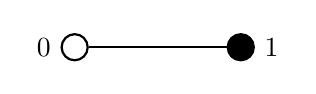
\begin{tikzpicture}[
            %scale=1,
            node distance=1.75cm,
            vblack/.style={circle,draw=black,fill=black,thick},
            vwhite/.style={circle,draw=black,fill=white,thick}
          ]
          \node[vwhite, label=left:$0$] (A) {};
          \node[right=of A, vblack, label=right:$1$] (B) {};
          \draw[thick] (A) to node [above] {} node {} (B);
        \end{tikzpicture}
      };

      % map
      \draw[black,->,thick] (dessin-top) to node [right] {$\varphi$} (dessin-bottom);
      %\draw[black,->] (dessin-top) -- (dessin-bottom);
      %\node at (19,18.75) {$X$};
      %\node at (19,5.25) {$\PP^1$};
      %\draw[black,->] (19,18)--(19,6);
    \end{tikzpicture}
\end{document}
